%!TEX root=main.tex

Esta heurística foi inspirada pelo guia estratégico~\cite{pentstrat}.

Há 4 formas de obter 5 em linha e ganhar um jogo de Pentago:
\begin{itemize}
	\item Monica - numa das diagonais principais do tabuleiro - força relativa 3
\begin{table}[H]
\centering
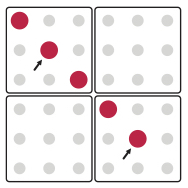
\includegraphics[height=3.7cm]{images/monica.jpg}
\end{table}
	\item Meio - na vertical ou na horizontal através do meio de dois quadrantes adjacentes - força relativa 5
\begin{table}[H]
\centering
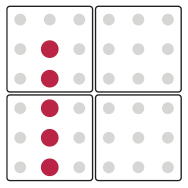
\includegraphics[height=3.7cm]{images/middle.jpg}
\end{table}
	\item Direito - na vertical ou na horizontal usando os bordos de dois quadrantes adjacentes - força relativa 7
\begin{table}[H]
\centering
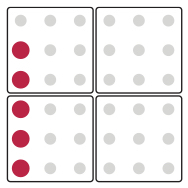
\includegraphics[height=3.7cm]{images/straight.jpg}
\end{table}
	\item Tripla - diagonalmente, abaixo ou acima das diagonais principais do tabuleiro - força relativa 9
\begin{table}[H]
\centering
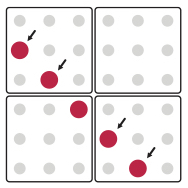
\includegraphics[height=3.7cm]{images/triple.jpg}
\end{table}
\end{itemize}

Para cada uma destas estratégias, considera-se a sua versatilidade, isto é, o número de diferentes possibilidades de aproveitar parte das peças quando um dos caminhos é bloqueado pelo adversário. Além disso, também nos interessa a dificuldade que o adversário tem de se defender contra um jogador que use a estratégia. São esses dois fatores que determinam a força relativa.

Dada uma posição do jogo, a heurística A começa por percorrer cada uma das linhas em que é possível ganhar e calcular o número de peças de cada cor. No entanto, apenas nos interessa contabilizar as peças quando há possibilidade do jogador conseguir ganhar nessa linha. Para isso, vamos verificar quantas peças há no interior da linha e quantas peças há nos bordos, dado que peças do adversário no interior bloqueiam imediatamente e para bloquear nos bordos são necessárias duas peças. Depois de efetuada esta contagem, sabemos quão forte é a posição de cada jogador em cada linha. Por exemplo, se há 3 peças brancas no interior e nenhuma peça preta em toda a linha, a posição branca é muito forte, porque basta mais uma peça para assegurar a sua vitória. 

No passo seguinte, usamos as forças relativas e as contagens para calcular o valor do tabuleiro. Sendo~$b$ o número de peças brancas,~$p$ o número de peças pretas e~$r$ a força relativa na linha em questão, adicionamos~$r^b - r^p$ ao valor previamente calculado. Este valor está a ser calculado assumindo que a IA está a jogar com as peças brancas, mas caso esteja a jogar com as pretas, basta multiplicar por -1 no final. O motivo pelo qual usamos a potência, é para garantir que ter várias peças na mesma linha é mais valorizado do que ter as mesmas peças espalhadas por linhas diferentes.

O método acima é usado para calcular o valor de todos os 8 tabuleiros que se obtém do tabuleiro atual por rotação de um quadrante. Depois disso, é usado o máximo ou o mínimo destes tabuleiros rodados, consoante o próximo jogador é a IA ou o adversário, tal como no minmax.

Em relação às forças relativas, apesar de querermos favorecer determinadas estratégias em detrimento de outras, não usamos os valores 3, 5, 7, e 9, porque devido ao uso de potências, eles conduzem a discrepâncias enormes entre jogadas, que fariam com que algumas das estratégias fossem completamente desprezadas. Sendo assim, após alguns cálculos com várias posições de jogo, optamos pelos valores 1.13, 1.15, 1.17 e 1.19. Isto contribui também para que os valores finais do tabuleiro sejam pequenos, o que será usado noutras considerações da heurística como veremos adiante. Dada a arbitrariedade da escolha dos valores, decidimos efetuar experiências estatísticas para determinar os melhores valores, mas isso será visto mais adiante na secção das experiências.

Observando jogos em que a heurística A perdia, rapidamente conseguimos determinar algumas das suas falhas. A primeira destas observações é que se um jogador conseguir 4 em linha com as duas pontas abertas (em jogadas do tipo monica, meio ou direito), então irá ganhar na próxima jogada, a não ser que o seu adversário ganhe já nesta. Assim, ao detetar estas situações a heurística A ignora todos os outros cálculos e dá valor 100 ao tabuleiro se ganha e -100 se perde.

Outra maneira certa de ganhar é conseguir duas ou mais linhas em que apenas falta uma peça para ganhar. Estas situações também foram introduzidas como exceção na heurística A, embora possam levar a alguns falsos positivos, quando ambas as linhas de vitória necessitam de uma peça na mesma posição do tabuleiro.

Finalmente, fizemos ainda algumas pequenas alterações aos valores da heurística:
\begin{itemize}
	\item se tivermos 4 peças em linha com as pontas abertas, mas for a vez do adversário, calculamos o valor como se fossem 10 peças, para que seja claramente mais valorizada que as restantes;
	\item se faltar apenas uma peça para obter 5 em linha e não estivermos na situação anterior, incrementamos a contagem de peças em 1;
	\item se houver 1, 2 ou 3 peças não bloqueadas na mesma linha (monica, meio ou direito), como ambas as pontas abertas, incrementamos a contagem em 1.
\end{itemize}